\section{Trabajando con texto}


\subsection{Fuentes}

La propiedad \textbf{font-family} (familia de fuentes) de CSS permite establecer la fuente (tipo de letra) de un elemento o etiqueta. La \textit{Tabla \ref{tab: 1}} contiene los dos tipos de familias de fuentes:
\begin{table}[H]
    \centering
    \caption{Tipos de familias de fuentes}
    \label{tab: 1}
    \begin{tabular}{c c}
        \hline
        \textbf{Generic family} & \textbf{Font family} \\
        \hline
        \multirow{2}{5cm}{Serif}                & Times New Roman \\
        & Georgia \\
        \multirow{2}{5cm}{Sans - serif}  & Arial \\
        & Verdana \\
        \multirow{2}{5cm}{Monospace}     & Courier New \\
        & Lucida Console \\
        \hline
    \end{tabular}
\end{table}

Las \textbf{familias genéricas} (o generic family) son un grupo de familias de fuentes, es decir, un grupo de fuentes, mientras que la familia de fuentes (o family font) es una fuente o tipo de letra que se puede utilizar.

Asignemos algunas fuentes a algunos párrafos y veamos el resultado en la \textit{Figura \ref{fig: 3}}:
\begin{lstlisting}
estilos.css
    /* Define distintas clases que almacenan las distintas fuentes. */
    .serif {
        /* Si fuente "Times New Roman" no está disponible, prueba con Times, si
         esta tampoco, con alguna parecida de la familia serif. */
        font-family: "Times New Roman", Times, serif;
    }
    .sansserif {
        font-family: Helvetica, Arial, sans-serif;
    }
    .monospace {
        font-family: "Courier New", Courier, monospace;
    }
    .cursive {
        font-family: Florence, cursive;
    }
    .fantasy {
        font-family: Blippo, fantasy;
    }
    .systemui {
        font-family: system-ui, -apple-system, BlinkMacSystemFont, 'Segoe UI', Roboto, Oxygen, Ubuntu, Cantarell, 'Open Sans', 'Helvetica Neue', sans-serif;
    }

prueba.html
    <p class="serif">Escrito con Serif.</p>
    <p class="sansserif">Escrito con Sans-Serif.</p> 
    <p class="monospace">Escrito con Monospace.</p> 
    <p class="cursive">Escrito con Cursive.</p> 
    <p class="fantasy">Escrito con Fantasy.</p>
    <p class="systemui">Escrito con System UI.</p>
\end{lstlisting}
\begin{figure}[H]
    \centering
    \caption{Uso de fuentes}
    \label{fig: 3}
    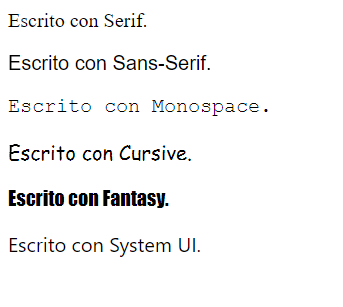
\includegraphics[width=6cm]{ss/fuentes.png}
\end{figure}

Como podemos ver, en el ejemplo anterior, si la fuente que deseamos no está disponible, podemos cargar otra deseada, si tampoco está disponible, podemos probar con alguna similar dentro de una familia, separado por comas (,); el ejemplo solamente prueba con dos fuentes antes de acudir a una familia, pero pueden ser más (no olvide que los nombres que son escritos con más de una palabra deben ser encerrados entre dobles comillas).

Una buena práctica es asignarle a todo el sitio web (body) una fuente genérica de respaldo, es decir, si queremos que todo nuestro sitio tenga la fuente de Google, pero por algún motivo, esta no está disponible (por la misma empresa o por una falla con el internet o máquina del cliente), podamos cargar otra fuente deseada y evitar un error de lectura. Lo anterior se resuelve como lo vimos en el ejemplo, poniendo diversas fuentes separadas por comas, para al final, poner una familia genérica.


\subsection{Tamaño de fuente}

La propiedad \textbf{font-size} de CSS permite establecer el tamaño de fuente del texto de un elemento o etiqueta. Una de las formas de hacer grande o pequeña el tamaño de fuente es por medio de \textbf{palabras clave}, tales como:
\begin{itemize}
    \item \textbf{small} (\textbf{smaller}, \textbf{x-small}, \textbf{xx-small}).
    \item \textbf{medium}.
    \item \textbf{large} (\textbf{larger}, \textbf{x-larger}, \textbf{xx-larger}).
    \item \textbf{inherit}, \textbf{initial} y \textbf{unset}.
\end{itemize}

Este método evita que el usuario varie el tamaño de la fuente, de esta forma, evitando que afecte la apariencia del sitio web. Un ejemplo y su resultado (\textit{Figura \ref{fig: 4}}):
\begin{lstlisting}
estilos.css
    /* Define distintas clases con tamaño de fuente distintas. */
    .small {
        font-size: small;
    }
    .medium {
        font-size: medium;
    }
    .large {
        font-size: large;
    }
    .xlarge {
        font-size: x-large;
    }

prueba.html
    <p class="small">Escrito pequeño.</p>
    <p class="medium">Escrito mediano.</p> 
    <p class="large">Escrito grande.</p> 
    <p class="x-large">Escrito muy grande.</p>
\end{lstlisting}
\begin{figure}[H]
    \centering
    \caption{Cambiando el tamaño de fuente}
    \label{fig: 4}
    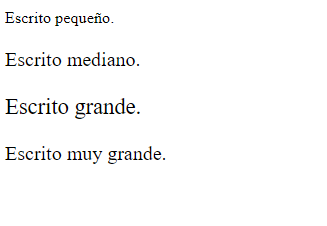
\includegraphics[width=6cm]{ss/fuentes-tam.png}
\end{figure}

La otra forma de definir el tamaño de fuente es mediante \textbf{Longitudes}: \textbf{px}, \textbf{em} o \textbf{porcentaje} (\%), la primera permite precisión en cuanto a píxeles en pantalla, mientras que la segunda permite cambio de tamaño en buscadores, pruebe ambas longitudes con zoom en su buscador para ver cómo funcionan y si se mantienen legibles (recuerde que 1em es igual a píxeles/16).
\begin{center}
    \textit{
        // Ambos tamaños son el mismo. \\
        font-size: 20px; \\
        font-size: 1.25em; \\
    }
\end{center}


\subsection{Estilo de fuente}

La propiedad \textbf{font-style} (estilo de fuente) permite aplicar un estilo de letra a la fuente, los valores que acepta esta propiedad son:
\begin{itemize}
    \item \textbf{normal}: texto sin ningún tipo de estilo (ni negrita).
    \item \textbf{italic}: texto en cursiva (lo mismo que la etiqueta \textbf{i}).
    \item \textbf{oblique}: texto como \textit{italic}, pero un poco más redonda (no es soportada por algunos buscadores).
    \item \textbf{oblique \textit{$<$ángulo$>$}}: texto como \textit{italic}, pero se le puede añadir un ángulo de inclinación al texto, esta propiedad no es muy soportada por los buscadores, los valores que puede recibir van de -90 a 90 deg.
    \item \textbf{inherit}, \textbf{initial} y \textbf{unset}.
\end{itemize}

Veamos un ejemplo y su resultado (\textit{Figura \ref{fig: 5}}):
\begin{lstlisting}
estilos.css
    /* Define distintas clases con estilos de fuente distintas. */
    .normal {
        font-style: normal;
    }
    .italic {
        font-style: italic;
    }
    .oblique {
        font-style: oblique;
    }

prueba.html
    <p class="normal">Escrito normal.</p>
    <p class="italic">Escrito italic.</p>
    <p class="oblique">Escrito oblique.</p>
\end{lstlisting}
\begin{figure}[H]
    \centering
    \caption{Cambiando el estilo de fuente}
    \label{fig: 5}
    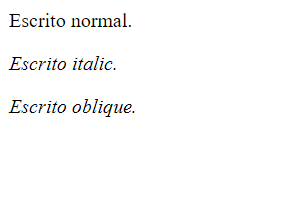
\includegraphics[width=6cm]{ss/fuentes-style.png}
\end{figure}

¿Porqué requeriría de esto si ya lo puedo conseguir con las etiquetas de HTML?, bueno, podemos aplicar un estilo de fuente distinto dinámicamente, por ejemplo, al dar un clic en un botón, un texto pasa de negrita a normal, normal a cursiva, etc.


\subsection{Grosor de fuente}

La propiedad\textbf{font-weight} (peso de fuente literalmente) de CSS permite establecer el grosor de fuente del texto de un elemento o etiqueta. Acepta los siguientes valores:
\begin{itemize}
    \item \textbf{normal}: texto normal con grosor predeterminado.
    \item \textbf{bold}: texto con un grosor mayor a \textit{normal} (como la etiqueta \textbf{b} o \textbf{stronger}).
    \item \textbf{bolder}: texto con un grosor mayor a \textit{bold}.
    \item \textbf{lighter}: texto con grosor menor a \textit{normal}.
    \item \textbf{inherit}, \textbf{initial} y \textbf{unset}.
\end{itemize}

Veamos un ejemplo y su resultado (\textit{Figura \ref{fig: 6}}):
\begin{lstlisting}
estilos.css
    /* Define distintas clases con grosores de fuente distintas. */
    .lighter {   
        font-weight: lighter;
    }
    .bold {   
        font-weight: bold;
    }
    .bolder {
        font-weight: bolder;
    }

prueba.html
    <p class="lighter">Escrito lighter.</p>
    <p class="bold">Escrito bold.</p>
    <p class="bolder">Escrito bolder.</p>
\end{lstlisting}
\begin{figure}[H]
    \centering
    \caption{Cambiando el grosor de fuente}
    \label{fig: 6}
    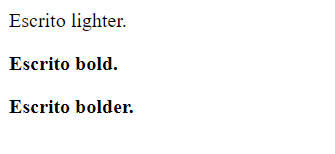
\includegraphics[width=6cm]{ss/fuentes-weight.png}
\end{figure}

Esta propiedad puede ser definida con valores enteros del 100 (ligero) a 900 (grueso), de acuerdo a como lo necesitemos. El valor 400 tiene el mismo grosor que el valor \textit{normal}, mientras que 700 tiene el mismo grosor que el valor \textit{bold}.
\begin{lstlisting}
    estilos.css
    /* Define distintas clases con grosores de fuente en valores. */
    .ligerito {   
        font-weight: 300;
    }
    .gruesesote {   
        font-weight: 850;
    }
\end{lstlisting}


\subsection{Variación de fuente}

La propiedad \textbf{font-variant} (variación de fuente) de CSS permite encoger ligeramente un texto de un elemento o etiqueta. Acepta los siguientes valores:
\begin{itemize}
    \item \textbf{normal}: texto con tamaño y estilo predeterminado.
    \item \textbf{small-caps}: texto encogido ligeramente y lo pasa a mayúsculas, tiene otros parámetros consecuentes que afectan al resultado final.
    \item \textbf{common-ligatures}: texto con tamaño predeterminado, pero con un espacio mayor entre letra y letra, tiene otros parámetros consecuentes que afectan al resultado final.
    \item \textbf{inherit}, \textbf{initial} y \textbf{unset}.
\end{itemize}

Veamos un ejemplo y su resultado (\textit{Figura \ref{fig: 7}}):
\begin{lstlisting}
estilos.css
    /* Define distintas clases con variaciones de fuente distintas. */
    .normal {
        font-variant: normal;
    }
    .small {
        font-variant: small-caps;
    }

prueba.html
    <p class="normal">Escrito normal.</p>
    <p class="small">Escrito small-caps.</p>
\end{lstlisting}
\begin{figure}[H]
    \centering
    \caption{Cambiando la variación de fuente}
    \label{fig: 7}
    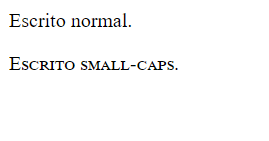
\includegraphics[width=6cm]{ss/fuentes-var.png}
\end{figure}


\subsection{Alineando texto horizontalmente}

La propiedad \textbf{text-align} de CSS permite establecer la alineación horizontal del texto de un objeto o etiqueta. Por defecto, el texto está alineado a la izquierda, pero también acepta los siguientes valores:
\begin{itemize}
    \item \textbf{start} o \textbf{left}: por defecto, alinea a la izquierda.
    \item \textbf{end} o \textbf{right}: alinea a la derecha.
    \item \textbf{center}: alinea al centro.
    \item \textbf{justify}: alinea a la izquierda y derecha.
    \item \textbf{inherit}, \textbf{initial} y \textit{unset}.
\end{itemize}

Veamos el siguiente ejemplo y su resultado (\textit{Figura \ref{fig: 8}}):
\begin{lstlisting}
estilos.css
    /* Define distintas clases con alineaciones de texto distintas. */
    .izq {
        text-align: left;
    }
    .der {
        text-align: right;
    }
    .cen {
        text-align: center;
    }
    .jus {
        text-align: justify;
    }

prueba.html
    <p class="izq">Lorem ipsum dolor sit amet, consectetur adipiscing elit, sed do eiusmod tempor incididunt ut
                labore et dolore magna aliqua. Ut enim ad minim veniam, quis nostrud exercitation ullamco laboris nisi ut
                aliquip ex ea commodo consequat</p>
    <p class="der">Lorem ipsum dolor sit amet, consectetur adipiscing elit, sed do eiusmod tempor incididunt ut
                labore et dolore magna aliqua. Ut enim ad minim veniam, quis nostrud exercitation ullamco laboris nisi ut
                aliquip ex ea commodo consequat</p>
    <p class="cen">Lorem ipsum dolor sit amet, consectetur adipiscing elit, sed do eiusmod tempor incididunt ut
                labore et dolore magna aliqua. Ut enim ad minim veniam, quis nostrud exercitation ullamco laboris nisi ut
                aliquip ex ea commodo consequat</p>
    <p class="jus">Lorem ipsum dolor sit amet, consectetur adipiscing elit, sed do eiusmod tempor incididunt ut
                labore et dolore magna aliqua. Ut enim ad minim veniam, quis nostrud exercitation ullamco laboris nisi ut
                aliquip ex ea commodo consequat</p>
\end{lstlisting}
\begin{figure}[H]
    \centering
    \caption{Cambiando la alineación de texto}
    \label{fig: 8}
    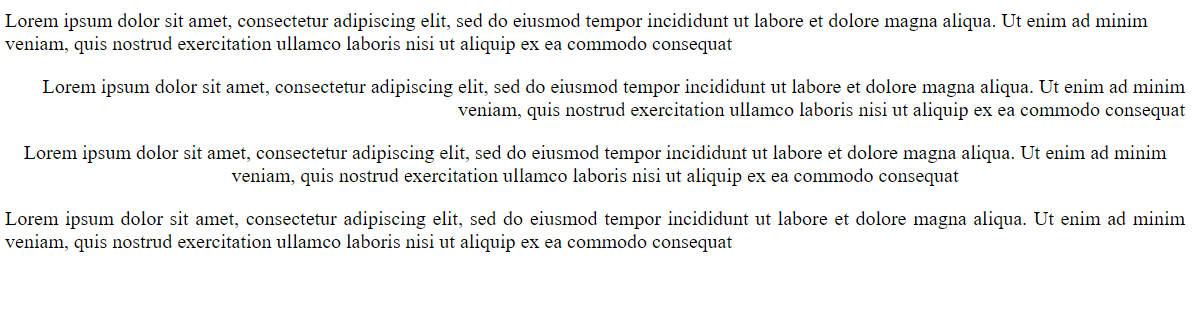
\includegraphics[width=14cm]{ss/fuentes-align.png}
\end{figure}


\subsection{Alineando texto verticalmente}

La propiedad \textbf{vertical-align} de CSS permite establecer la alineación vertical del texto de un objeto o etiqueta. Por defecto, el texto está alineado en la parte superior de la página, pero también acepta los valores:
\begin{itemize}
    \item \textbf{top}: alinea el tope del elemento con el tope de la línea entera o su contenedor.
    \item \textbf{bottom}: alinea la base del elemento con la base de la línea entera o su contenedor.
    \item Valores con respecto el elemento padre:
    \begin{itemize}
        \item \textbf{baseline}: alinea la base del elemento con la base de su elemento padre.
        \item \textbf{sub}: alinea la base del elemento con la base del subíndice de su elemento padre.
        \item \textbf{super}: alinea la base del elemento con la base del superíndice de su elemento padre.
        \item \textbf{text-top}: alinea el tope del elemento con el tope de la letra de su elemento padre.
        \item \textbf{text-bottom}: alinea la base del elemento con la base de la letra de su elemento padre.
        \item \textbf{middle}: alinea la mitad del elemento con la base más una porción X del alto de su elemento padre.
    \end{itemize}
    \item \textbf{inherit}, \textbf{initial} y \textit{unset}.
\end{itemize}

Veamos el siguiente ejemplo con una tabla y su resultado (\textit{Figura \ref{fig: 9}}):
\begin{lstlisting}
estilos.css
    /* Define distintas clases con alineaciones verticales de texto distintas. */
    .cima {
        vertical-align: top;
    }
    .medio {
        vertical-align: middle;
    }
    .fondo {
        vertical-align: bottom;
    }

prueba.html
    <table border="1" cellpadding="2" cellspacing="0" style="height: 150px;">
        <tr>
            <td class="cima">Top</td>
            <td class="medio">Middle</td>
            <td class="fondo">Bottom</td>
        </tr>
    </table>
\end{lstlisting}
\begin{figure}[H]
    \centering
    \caption{Cambiando la alineación vertical de texto 1}
    \label{fig: 9}
    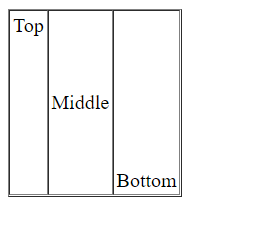
\includegraphics[width=5cm]{ss/fuentes-align-v1.png}
\end{figure}

Lamentablemente, los palabras clave anteriormente mencionadas solamente aplican para las etiquetas \textbf{table}, sin embargo, podemos utilizar otras palabras reservadas como valores para otras etiquetas con esta propiedad, los cuales son: \textbf{baseline}, \textbf{sub}, \textbf{super} y \textbf{Longitudes} (\%, px, pt, cm, em, etc.). Veamos un ejemplo continuación (\textit{Figura \ref{fig: 10}}).
\begin{lstlisting}
estilos.css
    /* Define distintas clases con alineaciones verticales de texto distintas. */
    .baseline {
        vertical-align: baseline;
    }
    .sub {
        vertical-align: sub;
    }
    .super {
        vertical-align: super;
    }
    .pixel {
        vertical-align: 10px;
    }

prueba.html
    <p>Este texto tiene una palabra <span class="baseline">baseline</span>.</p>
    <p>Este texto tiene una palabra <span class="sub">sub</span>.</p>
    <p>Este texto tiene una palabra <span class="super">super</span>.</p>
    <p>Este texto tiene una palabra <span class="pixel">subida 10 píxeles</span>.</p>
\end{lstlisting}
\begin{figure}[H]
    \centering
    \caption{Cambiando la alineación vertical de texto 2}
    \label{fig: 10}
    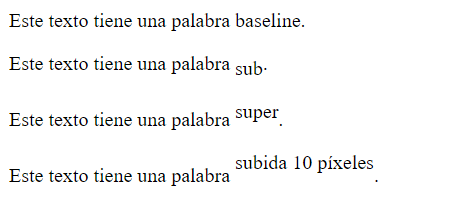
\includegraphics[width=9cm]{ss/fuentes-align-v2.png}
\end{figure}

\textit{Nota}: el ejemplo anterior aplicó a un párrafo (\textbf{p} y \textbf{span}), pero requiere de más instrucciones (propiedades) para otras etiquetas.


\subsection{Color de texto}

La propiedad \textbf{color} de CSS permite establecer un color determinado al texto de un objeto o etiqueta. Una de las formas de aplicar color al texto es utilizando las palabras claves con los nombres de los colores, por ejemplo: \textit{red}, \textit{green}, \textit{blue}, etc. Veamos un ejemplo rápido (\textit{Figura \ref{fig: 11}}):
\begin{lstlisting}
estilos.css
    /* Define una clase que asigna el color rojo al texto. */
    .colores {
        color: red;
    }

prueba.html
    <p class="colores">Escrito con color rojito.</p>
    <p>Escrito con el color predefinido (negro).</p>
\end{lstlisting}
\begin{figure}[H]
    \centering
    \caption{Cambiando el color del texto}
    \label{fig: 11}
    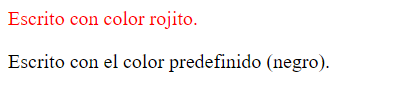
\includegraphics[width=9cm]{ss/fuentes-color.png}
\end{figure}

La otra forma de asignar colores es por medio de valores hexadecimales, compuesto por un \# al inicio y seis caracteres, que van de o a F, o RGB, que define un valor de 0 a 255 para el rojo, verde y azul (Red, Green y Blue).
\begin{center}
    \textit{
        // Color blanco. \\
        color: \#FFFFFF; \\
        color: rgb(255, 255, 255); \\
    }
\end{center}


\subsection{Decoración del texto}

La propiedad \textbf{text-decoration} de CSS permite establecer una decoración al texto de un objeto o etiqueta. Algunos de los valores aceptados son:
\begin{itemize}
    \item \textbf{none}: establece un texto regular o normal, sin estilo ni decoración.
    \item \textbf{overline}: establece una línea horizontal encima del texto.
    \item \textbf{underline}: establece una línea horizontal debajo del texto.
    \item \textbf{line-through}: establece una línea horizontal en medio del texto, es decir, lo tacha (sustituye la etiqueta \textbf{s} de HTML).
    \item \textbf{inherit}, \textbf{initial} y \textit{unset}.
\end{itemize}

Veamos un ejemplo rápido (\textit{Figura \ref{fig: 12}}):
\begin{lstlisting}
estilos.css
    /* Define una clase que asigna una decoración al texto distinta. */
    .none {
        text-decoration: none;
    }
    .inherit {
        text-decoration: inherit;
    }
    .overline {
        text-decoration: overline;
    }
    .underline {
        text-decoration: underline;
    }
    .line-through {
        text-decoration: line-through;
    }
    
prueba.html
    <p class="none">Escrito predeterminado.</p>
    <p class="inherit">Escrito que hereda el estilo de su padre.</p>
    <p class="overline">Escrito que tiene una línea encima.</p>
    <p class="underline">Escrito que tiene una línea debajo.</p>
    <p class="line-through">Escrito que está tachado.</p>
\end{lstlisting}
\begin{figure}[H]
    \centering
    \caption{Cambiando la decoración del texto}
    \label{fig: 12}
    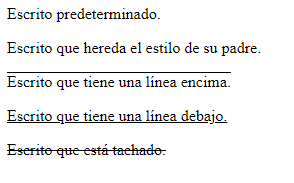
\includegraphics[width=9cm]{ss/fuentes-deco.png}
\end{figure}

Esta propiedad tiene otras propiedades consecuentes, como lo son un color, estilo o grosor, por ejemplo:
\begin{center}
    \textit{text-decoration: underline dotted red;}
\end{center}

Los \textbf{colores} ya sabemos que pueden ser utilizamos mediante palabras reservadas o códigos hexadecimales, los valores para la propiedad \textbf{estilo} son similares o iguales a los valores utilizados para estilizar los bordes de tablas (\textit{dotted}, \textit{solid}, \textit{double}, etc), los valores para la propiedad \textbf{grosor} son \textbf{auto} y \textbf{from-font}.


\subsection{Indentación del texto}

La propiedad \textbf{text-indent} de CSS permite establecer una indentación al texto de un objeto o etiqueta. Acepta \textbf{Longitudes} como valor para definir el espacio del lado izquierdo antes de comenzar el texto (px, pt, cm, em, \%, \textbf{inherit}, \textbf{initial} y \textbf{unset}, valores negativos, etc.). Veamos un ejemplo rápido (\textit{Figura \ref{fig: 13}}):
\begin{lstlisting}
estilos.css
    /* Define una clase que asigna una indentación al texto. */
    p {
        text-indent: 20px;
    }
    
prueba.html
    <p>Lorem ipsum dolor sit amet, consectetur adipiscing elit, sed do eiusmod tempor 
            incididunt ut labore et dolore magna aliqua. Ut enim ad minim veniam, quis 
            nostrud exercitation ullamco laboris nisi ut aliquip ex ea commodo consequat</p>
\end{lstlisting}
\begin{figure}[H]
    \centering
    \caption{Cambiando la indentación del texto}
    \label{fig: 13}
    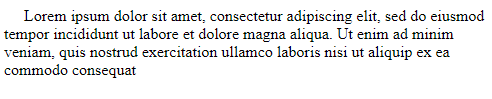
\includegraphics[width=12cm]{ss/fuentes-indent.png}
\end{figure}


\subsection{Sombra del texto}

La propiedad \textbf{text-shadow} de CSS permite establecer una sombra proveniente del centro del texto de un objeto o etiqueta. Posee cuatro parámetros: distancia del centro del texto con respecto al eje X (horizontal), distancia del centro del texto con respecto al eje Y (vertical), lo borroso o difuminado de la sombra y su color; todos estos parámetros \textbf{no} van separados por comas. Veamos un ejemplo rápido (\textit{Figura \ref{fig: 14}}):
\begin{lstlisting}
estilos.css
    /* Define una clase que asigna una una sombra con color al texto. */
    .sombrita {
        color: blueviolet;
        /* La sombra se proyecta en diagonal 5 y 5 píxeles hacía la abajo y derecha,
           está difuminada 5 píxeles y es de color azul. */
        text-shadow: 5px 5px 5px blue;
    }
    
prueba.html
    <h1 class="sombrita">Este texto tiene sombra</h1>
\end{lstlisting}
\begin{figure}[H]
    \centering
    \caption{Agregando sombra al texto}
    \label{fig: 14}
    
\includegraphics[width=7cm]{ss/fuentes-shadow.png}
\end{figure}

Como podemos suponer, los valores de los atributos pueden ser negativos y las distintas \textbf{Longitudes} permitidas por CSS, podemos utilizar valores hexadecimales o RGB para establecer el color de la sombra y podemos establecer múltiples sombras a un texto, simplemente separamos este grupo de parámetros por una coma y ponemos otro grupo de cuatro:
\begin{center}
    \textit{text-shadow: 5px 5px 5px blue, rgba(0,0,255,1) -1px -2px 0.5em;}
\end{center}

Un valor que también se puede poner es \textbf{transparent}, que hace transparente una sombra, además de \textbf{inherit}, \textbf{initial} y \textit{unset}.


\subsection{Transformación del texto}

La propiedad \textbf{text-transform} de CSS permite configurar la forma en la que aparecen las mayúsculas y minúsculas en el texto de un objeto o etiqueta. Algunos valores que acepta esta propiedad son:
\begin{itemize}
    \item \textbf{none}: aplica un estilo normal o predeterminado a un texto.
    \item \textbf{capitalize}: pone mayúsculas a cada palabra de un texto.
    \item \textbf{uppercase}: vuelve todo el texto mayúscula.
    \item \textbf{lowercase}: vuelve todo el texto minúscula.
    \item \textbf{inherit}, \textbf{initial} y \textit{unset}.
\end{itemize}

Veamos un ejemplo rápido (\textit{Figura \ref{fig: 15}}):
\begin{lstlisting}
estilos.css
    /* Define una clase que cambia el orden de minúsculas y mayúsculas del texto. */
    .none {
        text-transform: none;
    }
    .capitalize {
        text-transform: capitalize;
    }
    .uppercase {
        text-transform: uppercase;
    }
    .lowercase {
        text-transform: lowercase;
    }
    
prueba.html
    <p class="none">eScRiTO nONe</p>
    <p class="capitalize">eScRiTO CaPiTaLiZe</p>
    <p class="uppercase">eScRiTO upperCASE</p>
    <p class="lowercase">eScRiTO LOWERcase</p>
\end{lstlisting}
\begin{figure}[H]
    \centering
    \caption{Cambiando las mayúsculas y minúsculas del texto}
    \label{fig: 15}
    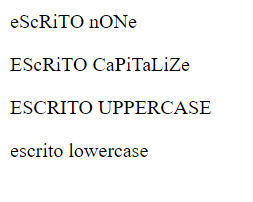
\includegraphics[width=5cm]{ss/fuentes-upper.png}
\end{figure}


\subsection{Espaciado entre letras}

La propiedad \textbf{letter-spacing} de CSS permite configurar el espaciado entre carácter y carácter de un texto de un objeto o etiqueta. Algunos valores que acepta esta propiedad son:
\begin{itemize}
    \item \textbf{normal}: no agrega ningún espaciado entre caracteres.
    \item \textbf{inherit}, \textbf{initial} y \textit{unset}.
\end{itemize}

Veamos un ejemplo rápido (\textit{Figura \ref{fig: 16}}):
\begin{lstlisting}
estilos.css
    /* Define una clase que cambia el espaciado de caracteres del texto. */
    .normal {
        letter-spacing: normal;
    }
    .esp {
        letter-spacing: 5px;
    }
        
prueba.html
    <p class="normal">Espaciado normal.</p>
    <p class="esp">Espaciado de 5px.</p>
\end{lstlisting}
\begin{figure}[H]
    \centering
    \caption{Cambiando el espaciado de caracteres del texto}
    \label{fig: 16}
    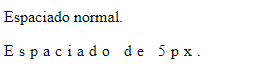
\includegraphics[width=7cm]{ss/fuentes-spacing.png}
\end{figure}

\textit{Nota}: letter-spacing acepta valores negativos.


\subsection{Espaciado entre palabras}

La propiedad \textbf{word-spacing} de CSS permite configurar el espaciado entre palabras de un texto de un objeto o etiqueta. Así como con la propiedad anterior, esta acepta los valores \textbf{normal}, una \textbf{Longitud} (\%, px, pt, cm, em, etc.), \textbf{inherit}, \textbf{initial} y \textit{unset}. Veamos un ejemplo rápido (\textit{Figura \ref{fig: 17}}):
\begin{lstlisting}
estilos.css
    /* Define una clase que cambia el espaciado de palabras del texto. */
    .normal {
        word-spacing: normal;
    }
    .esp {
        word-spacing: 20px;
    }
        
prueba.html
    <p class="normal">Este párrafo tiene un espaciado de palabras normal.</p>
    <p class="esp">Este párrafo tiene un espaciado de palabras de 20 píxeles.</p>
\end{lstlisting}
\begin{figure}[H]
    \centering
    \caption{Cambiando el espaciado de palabras del texto}
    \label{fig: 17}
    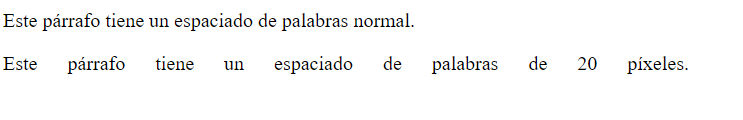
\includegraphics[width=14cm]{ss/fuentes-ws.png}
\end{figure}

\textit{Nota}: word-spacing acepta valores negativos.


\subsection{Manejo de espacios y saltos de línea}

La propiedad \textbf{white-space} de CSS permite configurar cómo son manejados los espacios en blanco y saltos de línea en textos, tanto en el código, como en el navegador cuando este cambia de tamaño, en otras palabras, maneja como se ajusta el texto cuando un elemento o etiqueta HTML sufre un cambio de tamaño Los valores que puede aceptar son los siguientes:
\begin{itemize}
    \item \textbf{normal}: el texto en código con secuencias de espacios y saltos de línea son reducidos a un solo espacio, manteniendo el texto dentro del espacio de la etiqueta que lo contiene.
    \item \textbf{nowrap}: trata los espacios y saltos de líneas como el valor \textit{normal}, pero el texto se sale del espacio de la etiqueta que lo contiene si esta no es lo suficientemente grande como para almacenarlo.
    \item \textbf{pre}: los múltiples espacios continuos se mantienen y los saltos de línea se dan con etiquetas \textbf{br} y con los caracteres de saltos de línea.
    \item \textbf{pre-wrap}: trata los espacios y saltos de líneas como el valor anterior, pero rellena con saltos de línea según sea necesario, para rellenar el contenedor que lo almacena.
    \item \textbf{pre-line}: trata los saltos de líneas como el valor anterior, pero la secuencia de espacios son reducidos a un solo espacio.
    \item \textbf{break-spaces}: idéntico al valor \textit{pre-wrap}, pero mantiene todos los espacios (incluidos los espacios al final de líneas) y secuencias de espacios.
\end{itemize}

La \textit{Tabla \ref{tab: 2}} muestra las diferentes situaciones donde podemos utilizar esta propiedad:
\begin{table}[H]
    \centering
    \caption{Usos de la propiedad \textit{white-space}}
    \label{tab: 2}
    \begin{tabular}{m{1.7cm} m{2cm} m{2.3cm} m{2cm} m{2cm} m{3cm}}
        \hline
        \parbox{1.7cm}{\raggedright} & \parbox{2cm}{\raggedright\textbf{Saltos de líneas}} & \parbox{2.3cm}{\raggedright\textbf{Espacios y \\tabulación}} & \parbox{2cm}{\raggedright\textbf{Ajuste de texto}} & \parbox{2cm}{\raggedright\textbf{Espacios al final}} & \parbox{3cm}{\raggedright\textbf{Separadores}} \\
        \hline
        \parbox{1.7cm}{\raggedright normal}       & \parbox{2cm}{\raggedright Se reducen} & \parbox{2.3cm}{\raggedright Se reducen} & \parbox{2cm}{\raggedright Se ajusta} & \parbox{2cm}{\raggedright Son removidos} & \parbox{3cm}{\raggedright Se cuelga} \\
        \hline
        \parbox{1.7cm}{\raggedright nowrap}       & \parbox{2cm}{\raggedright Se reducen}    & \parbox{2.3cm}{\raggedright Se reducen}    & \parbox{2cm}{\raggedright No se ajusta}  & \parbox{2cm}{\raggedright Son removidos} & \parbox{3cm}{\raggedright Se cuelga}    \\
        \hline
        \parbox{1.7cm}{\raggedright pre}          & \parbox{2cm}{\raggedright Se mantienen}  & \parbox{2.3cm}{\raggedright Se mantienen}  & \parbox{2cm}{\raggedright No se ajusta}  & \parbox{2cm}{\raggedright Se mantienen}  & \parbox{3cm}{\raggedright No se ajusta} \\
        \hline
        \parbox{1.7cm}{\raggedright pre-wrap}     & \parbox{2cm}{\raggedright Se mantienen}  & \parbox{2.3cm}{\raggedright Se mantienen}  & \parbox{2cm}{\raggedright Se ajusta}     & \parbox{2cm}{\raggedright Se cuelga}     & \parbox{3cm}{\raggedright Se cuelga}    \\
        \hline
        \parbox{1.7cm}{\raggedright pre-line}     & \parbox{2cm}{\raggedright Se mantienen}  & \parbox{2.3cm}{\raggedright Se reducen}    & \parbox{2cm}{\raggedright Se ajusta}     & \parbox{2cm}{\raggedright Son removidos} & \parbox{3cm}{\raggedright Se cuelga}    \\
        \hline
        \parbox{1.7cm}{\raggedright break-spaces} & \parbox{2cm}{\raggedright Se mantienen}  & \parbox{2.3cm}{\raggedright Se mantienen}  & \parbox{2cm}{\raggedright Se ajusta}     & \parbox{2cm}{\raggedright Se cuelga}     & \parbox{3cm}{\raggedright Se ajusta}    \\
        \hline
    \end{tabular}
\end{table}

Veamos un ejemplo rápido (\textit{Figura \ref{fig: 18}}):
\begin{lstlisting}
estilos.css
    /* Define una clase que manipula distinto los espaciados y saltos de líneas del texto. */
    /* Estilo de apoyo para visualizar mejor el ejemplo. */
    p {
        border-color: black;
        border-style: solid;
    }
    .normal {
        white-space: normal;
    }
    .nowrap {
        white-space: normal;
    }
    .pre {
        white-space: pre;
    }
    .pre-wrap {
        white-space: pre-wrap;
    }
    .pre-line {
        white-space: pre-line;
    }
    .break-spaces {
        white-space: break-spaces;
    }
        
prueba.html
    <p class="normal">Este párrafo             tiene
            un espaciado blanco              de palabras
            normal.
    </p>
    <p class="nowrap">Este párrafo             tiene
                un espaciado blanco              de palabras
                <i>nowrap</i>.
    </p>
    <p class="pre">Este párrafo             tiene
                 un espaciado blanco              de palabras
                  <i>pre</i>.
    </p>
    <p class="pre-wrap">Este párrafo             tiene
                un espaciado blanco              de palabras
                <i>pre-wrap</i>.
    </p>
    <p class="pre-line">Este párrafo             tiene
                un espaciado blanco              de palabras
                <i>pre-line</i>.
    </p>
    <p class="break-spaces">Este párrafo             tiene
                un espaciado blanco              de palabras
                <i>break-spaces</i>.
    </p>
\end{lstlisting}
\begin{figure}[H]
    \centering
    \caption{Cambiando el manejo de espacios y saltos de líneas del texto}
    \label{fig: 18}
    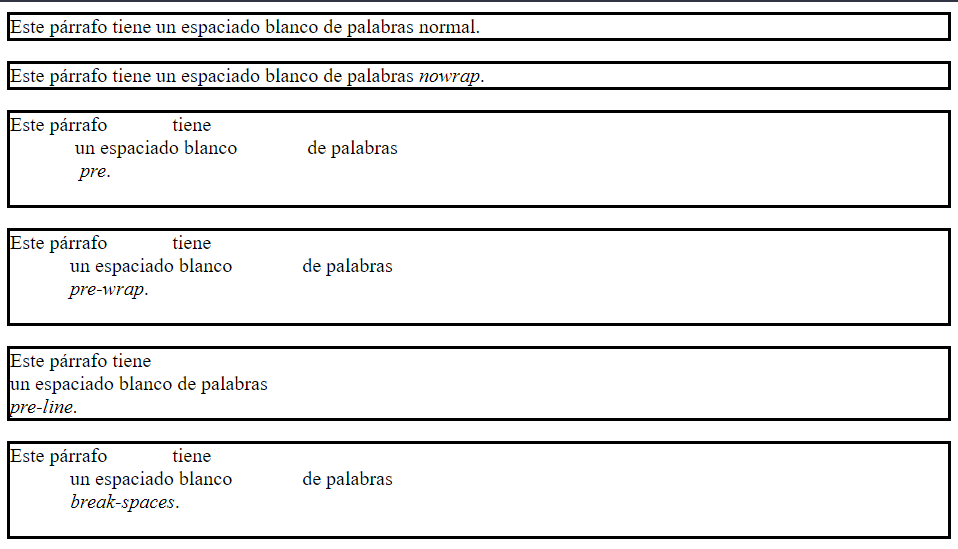
\includegraphics[width=14cm]{ss/fuentes-white-sp.png}
\end{figure}
